\documentclass[a4paper,10pt]{article}
\usepackage[utf8x]{inputenc}
\usepackage{graphicx}
\usepackage{color}
\usepackage{hyperref}
\usepackage[hmargin=3cm,vmargin=2.5cm]{geometry}
\usepackage{nameref}


% Meta data
\hypersetup {
    bookmarks=true,         % show bookmarks bar?
    unicode=false,          % non-Latin characters in Acrobats bookmarks
    pdftoolbar=true,        % show Acrobat's toolbar?
    pdfmenubar=true,        % show Acrobat's menu?
    pdffitwindow=false,     % window fit to page when opened
    pdfstartview={FitH},    % fits the width of the page to the window
    pdftitle={or-tools user's manual},    % title
    pdfauthor={Google},     % author
    pdfsubject={User's manual for the Google or-tools library},   % subject of the document
    pdfcreator={Google},   % creator of the document
    pdfproducer={Google}, % producer of the document
    pdfkeywords={or-tools} {open source} {constraint programming} {operations research}, % list of keywords
    %pdfnewwindow=true,      % links in new window
    colorlinks=true,       % false: boxed links; true: colored links
    linkcolor=blue,          % color of internal links
    citecolor=green,        % color of links to bibliography
    filecolor=magenta,      % color of file links
    urlcolor=cyan           % color of external links
}

\newcommand{\code}[1]{\texttt{#1}}

%opening
\title{How to generate the documentation for the or-tools library}
\author{Nikolaj van Omme\footnote{You can reach me at ortools.doc@gmail.com if you need some help. ;-) }}
\date{\today}

\begin{document}

\maketitle

\begin{abstract}
This little document explains how to generate and upload all the documentation for the Google or-tools library. This document doesn't explain how to write the documentation i.e. how to use of \emph{Sphinx}, \emph{Jinja2}, \emph{html}, \emph{css}, etc., only how to generate the output files once
the documentation is written and how to upload the output files on the Google servers. All the scripts are written in Python and must be called in the correct sequence.\\
\begin{center}\textcolor{red}{Only tested under Linux.}\end{center}
\begin{center}\textcolor{red}{THIS DOCUMENT IS NOT UP TO DATE AND CONTAINS ERRORS!}\end{center}
\end{abstract}

\setcounter{tocdepth}{2}
\tableofcontents

\section{Introduction (How it works)}

This documentation and the process to generate the or-tools library's documentation was designed with the or-tools people in mind. As such, the whole generation process isn't bullet-proof nor idiot-proof.\\

You can get your local copy of the documentation and generate it if you want but there is no reason to do so as all the generated documentation is already available on the Google servers. If you find better ways to generate some parts of the documentation, please share with the whole community (but keep in mind that our main purpose is not to spend too much time on this).\\

This document itself is written in~\LaTeX\ and generated with~PDF\LaTeX.

\subsection{Vocabulary}

To avoid misunderstanding, let's agree on some wordings.

\begin{description}
 \item[Source/Code file] a file in wich you write the documentation. It can be restructuredText (.rst), \LaTeX\ (.tex) or text (.txt, .css, html, \ldots)\footnote{Basically, \emph{all} source files are text files.}. Some files are at the same time source and output files.
 \item[Output file] a file that will be published on the server side, including html files, images, etc. Some files are at the same time source and output files.
 \item[Local home] the computer you use to write the documentation.
 \item[Google servers] the servers where the documentation is publicly accessible from the Internet.
 \item[Documentation hub] a central html page from which all the documentation is accessible except the downloadable files. The url is:\\
 \href{http://or-tools.googlecode.com/svn/trunk/documentation/documentation\_hub.html}{http://or-tools.googlecode.com/svn/trunk/documentation/documentation\_hub.html}.
\end{description}

\subsection{Directories}

There are seven main directories: four on the Local home side (\code{SOURCES}, \code{BUILD}, \code{DEPLOY} and \code{DOCUMENTATION}) and three on the Google servers side (\code{svn/doc\_sources}, \code{files} and  \code{svn/trunk/documentation}). Figure~\ref{pic_directories} illustrates those directories. The four local directories can be named to your liking (see section~\ref{installation}).

\begin{figure}[h]
   \centering
   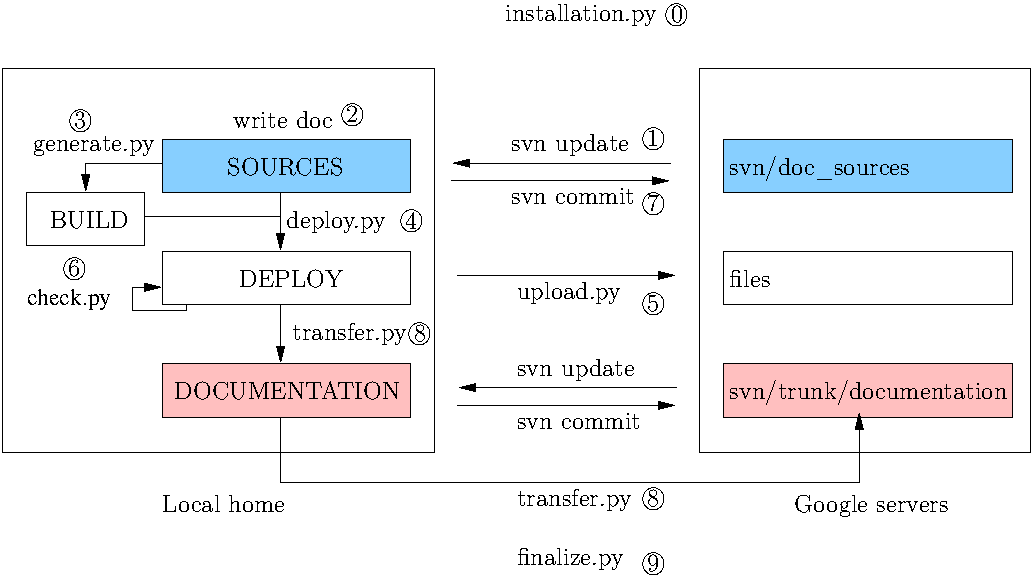
\includegraphics[scale=0.8]{images/directories.pdf}
   \caption{figure}{The six main directories and the scripts/commands to move the files between them. The base url for the Google Servers is~\href{http://or-tools.googlecode.com/}{http://or-tools.googlecode.com/}. The directories colored in the same color are svn copies of each other\footnotemark.}\label{pic_directories}
 \end{figure}

\begin{description}
 \item[\code{SOURCES}] This local directory contains the sources files, the scripts files and some configuration files. This directory is a local copy of the the directory \code{doc\_sources}.
 \item[\code{BUILD}] This local directory contains all the automatically generated output files. 
 \item[\code{DEPLOY}]  This local directory contains all the generated output files (automatically or by hand). It is not a local copy of the \code{trunk/documentation} directory as the directory structure is slightly different. We use it essentially for testing purpose.
 \item[\code{DOCUMENTATION}] The real thing, i.e. the documentation you can access from the documentation hub. This local directory is a local copy of the \code{trunk/documentation} directory. Actually, it is more the opposite: \code{svn/trunk/documentation} is a copy of your local directory \code{DOCUMENTATION} as we push (commit) the generated documentation on the Google servers without pulling (updating) it.
 \item[\code{svn/doc\_sources}] A server directory containing the sources files of the documentation. All the files you need to generate the documentation are stored in this directory. The full url is~\href{http://or-tools.googlecode.com/svn/doc\_sources}{http://or-tools.googlecode.com/svn/doc\_sources}.
 \item[\code{files}] A server directory containing the downloadable files. The full url is~\href{http://or-tools.googlecode.com/files}{http://or-tools.googlecode.com/files}. Note that you don't have public access to the directory, only to the files stored in it.
 \item[\code{svn/trunk/documentation}] A server directory with the or-tools library's documentation (except for the downloadable files). The full url is~\href{http://or-tools.googlecode.com/svn/trunk/documentation}{http://or-tools.googlecode.com/svn/trunk/documentation}.
\end{description}

\footnotetext{We don't consider white as a color, at least not in this document.} 

\subsection{Contents of the \code{SOURCES} directory}
\label{doc_content}

The documentation is explained on the documentation hub.\\

The local directory \code{SOURCES} contains the following files:

\begin{description}
 \item[\code{current\_version.txt}] Text file with the actual release number (xx.yy.zz), i.e. the release number of the next documentation you will upload.
 \item[\code{global.rst}] Rst file with global variables. You can update it manually if you need to.
 \item[\code{README.txt}] You know...
 \item[\code{TODO.txt}] What we plan for the future.
\end{description}

The local directory \code{SOURCES} contains the following directories:

\begin{description}
 \item[\code{doc}] The doc of the doc, i.e. the \LaTeX\ files to generate this document.
 \item[\code{FAQ}] Source files for the Frequently Asked Questions. The FAQ is generated by Sphinx.
 \item[\code{HUB}] Sources files for the documentation hub. Written by hand but with the help of the Python \code{generate.py} script.
 \item[\code{internals}] Internal files for the scripts. You shouldn't change anything here.
 \item[\code{LABS}] Exercises. 
\end{description}

\subsection{Work flow}

The whole process is divided in 9~steps\footnote{Once you get used to the documentation generation, you will be able to skip some of the steps (when you don't need to update the whole documentation tree) and to only use the specific manual commands you need.}. Most of the steps are automated by Python scripts and to simplify your life (and mine), several scripts are bundled in the global scripts (see section~\ref{global_scripts}). These scripts need to be called in sequence. In each of the subdirectories of the directory~\code{SOURCES} (see section~\ref{doc_content}), you will find the corresponding Python scripts if needed. If you don't 
find a specific script in a subdirectory, it means this script is not needed for that type of documentation.\\

\begin{description}
 \item[Step \raisebox{.3pt}{\textcircled{\raisebox{-.9pt} {1}}}] {\bf Update the source code:} (script: none)\\Update your local copy of the documentation via svn: \code{svn update}.
 \item[Step \raisebox{.3pt}{\textcircled{\raisebox{-.9pt} {2}}}] {\bf Write the documentation:} (script: none)\\Let your talent speak!
 \item[Step \raisebox{.3pt}{\textcircled{\raisebox{-.9pt} {3}}}] {\bf Generate the documentation:} (script: \code{generate.py})\\Generate automatically the documentation. You will find the generated documentation
in the \code{BUILD}~directory. For the moment (as of May 27 2012), only the manual (subdirectory~\code{MANUAL}) and the FAQ (subdirectory~\code{FAQ}) are automatically generated.\\
The documentation hub is parlty generated automatically, partly generated by hand. See section~\ref{generate_documentation_hub} for more details. 
 \item[Step \raisebox{.3pt}{\textcircled{\raisebox{-.9pt} {4}}}] {\bf Deploy the documentation:} (script: \code{deploy.py})\\Copy locally the output files in the directory~\code{DEPLOY}. This directory is used to test
the documentation and try new things without messing with the svn directory.
\item[Step \raisebox{.3pt}{\textcircled{\raisebox{-.9pt} {5}}}] {\bf Upload the documentation:} (script: \code{upload.py})\\Before you can check the documentation in the \code{DEPLOY}~directory, and if you want to test the download links, you have to upload the downloadable files. The \code{upload.py}~script will be stuck if you try to upload a file that is already uploaded (based on the filename). If you want to update a downloadable file, you first have to delete the file from the Google servers. For the moment, this action has to be done manually through web user interface. If you know how to do it with a script, we are interested!
 \item[Step \raisebox{.3pt}{\textcircled{\raisebox{-.9pt} {6}}}] {\bf Check the documentation:} (script: \code{check.py})\\Check the documentation. As of May 27 2012, the \code{check.py}~script only checks extern links. The rest is a manual (and important!) process.
 \item[Step \raisebox{.3pt}{\textcircled{\raisebox{-.9pt} {7}}}] {\bf Update the documentation source:} (script: none)\\If you're happy with the new documentation, commit your changes on the Google solvers. 
 \item[Step \raisebox{.3pt}{\textcircled{\raisebox{-.9pt} {8}}}] {\bf Upload the documentation:} (script: \code{transfer.py})\\Push (commit) the documentation on the Google servers. Prefer to use the \code{transfer.py}~script over the svn commands.
 \item[Step \raisebox{.3pt}{\textcircled{\raisebox{-.9pt} {9}}}] {\bf Prepare the next release of the documentation:} (script: \code{finalize.py})\\The documentation has a release number (xx.yy.zz). It is used internally by the scripts to check some operations. The \code{finalize.py}~script will copy the old number and update the new number (for instance, from 4.5.11 to 4.5.12 by default). You MUST use this script after step~\raisebox{.3pt}{\textcircled{\raisebox{-.9pt} {8}}}. If you want to update the release number to a higher release number, edit manually the file~\code{current\_version.txt} in the~\code{SOURCES} directory.
\end{description}

Section~\ref{generate_documentation} provides a more detailed account on how to generate the documentation.


\subsection{Preferred use}

These scripts are not bullet-proof nor idiot-proof. I strongly suggest that the source files always match the documentation files in~\href{http://or-tools.googlecode.com/svn/trunk/documentation}{http://or-tools.googlecode.com/svn/trunk/documentation} . Once you have finished steps \raisebox{.5pt}{\textcircled{\raisebox{-.9pt} {1}}} - \raisebox{.5pt}{\textcircled{\raisebox{-.9pt} {6}}}, commit your changes on the Google solvers (step \raisebox{.5pt}{\textcircled{\raisebox{-.9pt} {7}}}). If there is a conflict, start the whole process again later when the generated documentation is up to date and matches the sources files on the Google servers. One easy way to ensure the consistency between the source and the documentation is to delegate to one single person the upload and commitment of the documentation (steps \raisebox{.5pt}{\textcircled{\raisebox{-.9pt} {8}}} - \raisebox{.5pt}{\textcircled{\raisebox{-.9pt} {{9}}}}) (or to redesign the whole process ;-) ). This design ask for some discipline but I think it is manageable among Googlers.



\section{Install the documentation and the needed tools}
\label{installation}

To do.

\subsection{External libraries and tools}

The following list details all the libraries and tools that I use to generate the documentation. Most of them are written in Python.

\begin{description}
 \item[Sphinx] This is the main library. It transforms \verb+restucturedText+ into plenty of other formats.
 \item[Jinja2] 
 \item[\LaTeX] To generate the pdf version of the manual, we use \LaTeX{} and \verb+pdflatex+ (and of course, the classical \verb+makeindex+/\verb+mkindex+, \verb+bibtex+, \ldots).
 \end{description}

We use also Python (2.7), make, html, css, ...

\subsection{Scripts}
The Python scripts are not bullet-proof.\\

% There are three main directories:
% \begin{description}
%  \item[SOURCES] contains all the sources. This is the directory where you write the documentation. This directory is located in the \verb+or-tools/documentation/SOURCES+ directory of the project.
%  \item[DEPLOY] is an ``exact'' copy of the \verb+or-tools/trunk/documentation+ directory. Some directories/files are only present as links (for instance \verb+reference_manual+).
%  \item[SVN] is an exact copy of the \verb+or-tools/trunk/documentation+ directory.
%  \end{description}
% 
% I use the directory~\verb+DEPLOY+ as an intermediate directory to be able to test some new stuff without polluting \verb+SVN+.\\
% 


% \begin{description}
%  \item[Step 1] \verb+deploy.py+ generates and copies the documentation to directory~\verb+DEPLOY+. It is also responsible for the generation of all needed files and repertories.
%  \item[Step 2] \verb+upload.py+ uploads certain files to the \verb+download+ directory of the or-tools project and copies the documentation to directory~\verb+SVN+. Along the way, this script generates the list of
% 	       \verb+svn+ commands in \verb+snv_commands_xxx.txt+ and this is the \textbf{only} file that it generates.
%  \item[Step 3] \verb+svn+: the traditional \verb+svn+ commands.
%  \end{description}

\section{or-tools Sphinx extension}

To do.

\section{Add to the manual~\ldots}
\label{write_documentation}

To do.

This section covers only the manual. To correct or add some material, just open the corresponding~\code{rst} file, follow the~\code{rst} syntax and the more specialized~\code{Sphinx} syntax and adapt the file to your needs. If you want to add a chapter or a section, read the next two sections. We discuss also how to add a label and a reference in section~\ref{adding_ref} and the front material as it requires a special treatment.

\subsection{a part}

\subsection{a chapter}
To add a chapter, follow the next steps:
\begin{enumerate}
 \item In \code{SOURCES/MANUAL/source/manual}, create a file \code{mychapter.rst} and a folder \code{mychapter} where you will write the different sections of the chapter. See the other \code{rst} files.
 \item Add an entry in \code{index.rst} in the table of contents at the end. This will add you chapter to the manual but will not make it visible yet.
 \item Update manually the table of contents and possibly renumber the other chapters:
       \begin{itemize}
        \item In \code{index.rst}, update the sidebar (\code{.. sidebar:: Content at a glance});
        \item In \code{MANUAL/source/doctemplates}, update \code{myglobaltoc.html}.This file is used to generate the toc in the sidebar for the first page of each chapter in the~\code{html}~version.
       \end{itemize}
 \item To make you chapter visible, open~\code{config.py} and update~\code{html\_sidebars} accordingly.
\end{enumerate}

There is nothing more to do for the~\LaTeX\ version.

\subsection{a section}

Just write your section in a~\code{rst} file in the folder corresponding to the chapter and add an entry in the corresponding~\code{rst} file of the chapter.

% \subsection{To add a label and a reference}
% \label{adding_ref}
% 
% Use the~\code{rst} syntax: \code{.. \_myreference:}. To refer to this reference, unfortunately, you have to produce two versions: one for the~\code{html} version and one for the~\LaTeX~version.\\
% 
% Here is an example:\\
% 
% \begin{verbatim}
% ..  _myreference:
% 
% Mysection
% ---------
% 
% Text text text text text text ...
% 
% ..  raw:: latex
% 
%     You can find more in section~\ref{manual/chaptername/filename_without_extension:myreference}
%     ...
% 
% ..  only:: html
% 
%     In :ref:`Mysection <myreference>`, we cover ... in more details.
% \end{verbatim}
% 
% 
% This duplication is needed because references are treated differently in the~\code{pdf} manual and the~\code{html} version. In the~\code{pdf} manual, you refer by the corresponding numbers (like this: You can find more in section~\ref{adding_ref}~\ldots) while in~\code{html}, your refer with the title name and a link (like this: In~\nameref{adding_ref}, we cover~\ldots\ in more details).\\
% 
% See the gotchas about some references and how~\code{Sphinx} transforms them.

\subsection{Front material}

Again, we have duplicated the text as~\code{Sphinx} treats the~\code{pdf} and~\code{html} versions differently.

\subsubsection{Title page}

\subsubsection{Foreword}

\subsubsection{Table of contents}

\section{Generate the documentation}
\label{generate_documentation}

\subsection{The manual}

\subsubsection{\emph{Final} or~\emph{draft} release}
\label{final_draft_mode}

\subsection{The documentation hub}
\label{generate_documentation_hub}

\subsection{The tutorial code}

\subsection{The slides}

\subsection{The version}
All the automatic generation of the doc is based on the current version number, so don't mess with it\footnote{An assert-like script is run by all the other scripts to verify that at least the current version is
greater than the version before.}! ;-) 
The file~\verb+current_version.txt+ contains the current version (the one that you will upload on the server). You can update it by hand. By default, after a deploy and an update, the next version is incremented by~$1$. For instance, if the current version was~\verb+1.2.23+ before deploying and updating, then the next version will be automatically set to~\verb+1.2.24+.\\

Each documentation of subdirectory \verb+SOURCES+  has an individual \verb+deploy_xxx+ and \verb+upload_xxx+ than can be called manually if desired. Pay attention to the order in which you call them.
 We detail each of them in the right sequence in the next subsections.
\subsection{Documentation Hub}

\subsubsection{The change files/directory}

\begin{description}
 \item[changes.txt] This is where you write what changed since the last upload of the documentation. This file is automatically inserted in \verb+documentation_hub.html+ so be carefull! ;-) Lines starting with \verb+#+ are comments that are not written in the html file. Don't add the version, this is done automatically. Note that this file is not automatically updated. You are responsible for its content.
 \item[changes\_list.txt] This file is automatically updated with the content of \verb+changes.txt+.
 \item[changes] This directory contains copies of all the \verb+changes.txt+ files.
 \end{description}

\section{Global cripts}
\label{global_scripts}


\section{Gotchas}

\begin{itemize}
 \item When in draft mode (see~\ref{final_draft_mode}), the section numbers in the html pages are wrong. 
 \item \LaTeX\ slides files have to start with \code{\textbackslash documentclass\{\}} on the first line (required by \code{generate\_slides.py}).
 \item Manual: the preface is copied once. This is necessary as Sphinx doesn't allow to differentiate between titles in \LaTeX\ and Sphinx.
 \item There is no automatic update between the Getting started page of the wiki and the one of the manual. If you change one, you have to change the other manually. 
 \item When you want to use class names in titles and want to talk about them in the plural, you have to add ~\verb+\s+, not just~\verb+s+:
  \begin{verbatim}
``SearchMonitor``\s
-------------------
  \end{verbatim}

  \item Capitalized letters in a reference become lower letters and dashes ("-") become underscores ("\_") in the~\LaTeX\ version of the references. So for instance, if the reference in your~\code{rst} file \code{my\_file.rst} in the directory~\code{manual/my\_chapter/} is~\code{MyStrange\_referenceIa}, the~\LaTeX~reference will be~\code{manual/my\_chapter/my\_file:mystrange-referenceia}. 
\end{itemize}

\section{Resources}

\subsection{Images}
\begin{description}
 \item[Xfig]
 \item[fig2pdf]
 \end{description}


\end{document}
